\section{Activity Forecasting}

\begin{frame}
	\frametitle{A Realistic Example}
	
	\begin{center}
		\begin{tikzpicture}
			\node at (0,0) [draw=white,ultra thick,inner sep=0pt]
			{
				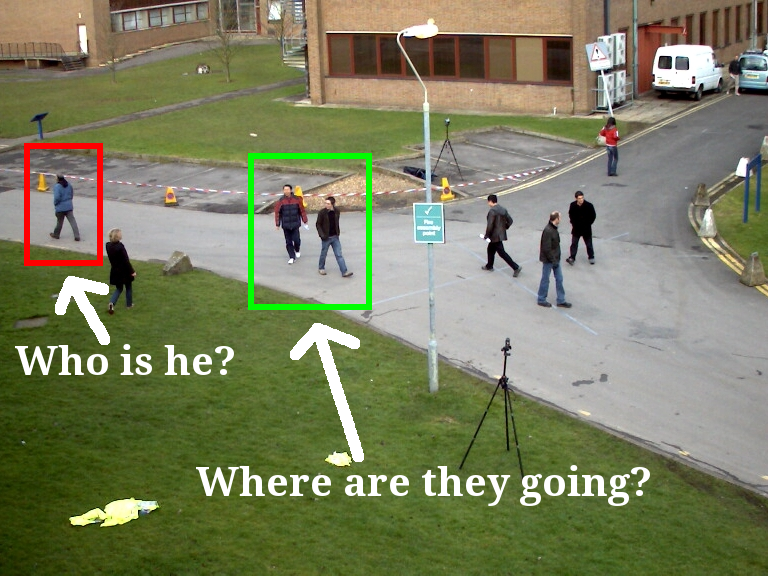
\includegraphics[scale=0.12]{Figures/Problem.png}
			};
		\end{tikzpicture}
	\end{center}
\end{frame}

\begin{frame}
	\frametitle{Activity Forecasting through Semantic Mapping}
	
	\vspace{0.7cm}
	
	\large
	
	Ziebart \emph{et al.} proposed a method for activity forecasting by combining
	
	\begin{itemize}
		\item Semantic scene understanding
		\vspace{0.05cm}
		\item Inverse Reinforcement Learning
	\end{itemize}
	
	\begin{center}
		\begin{tikzpicture}
			\node at (0,0) [draw=white,ultra thick,inner sep=0pt]
			{
				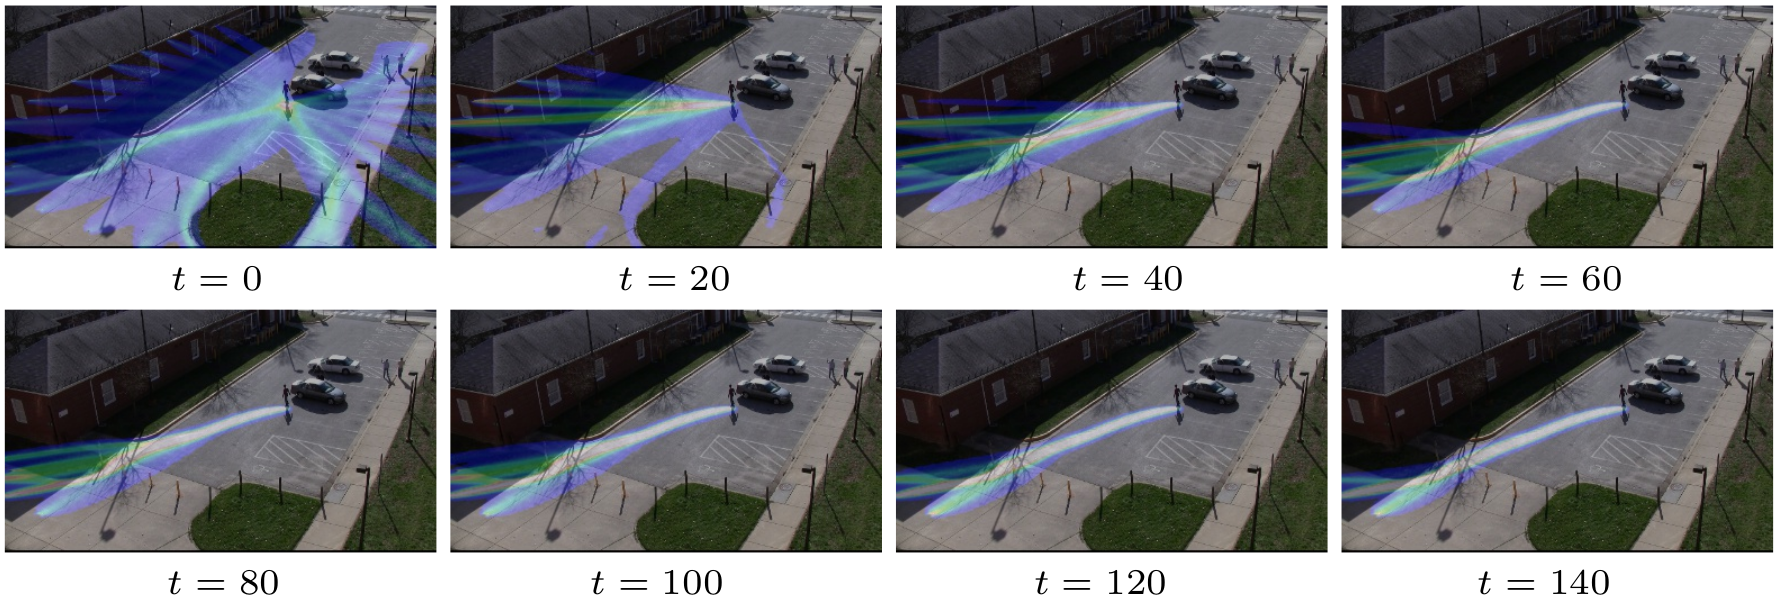
\includegraphics[scale=0.19]{Figures/ActivityForecasting.png}
			};
		\end{tikzpicture}
	\end{center}
\end{frame}

\begin{frame}
	\frametitle{Trajectory-Based IRL for Activity Forecasting}
	
	\vspace{0.13cm}
	
	\begin{center}
		\begin{tikzpicture}
			\node at (0,0) [draw=black,ultra thick,inner sep=0pt]
			{
				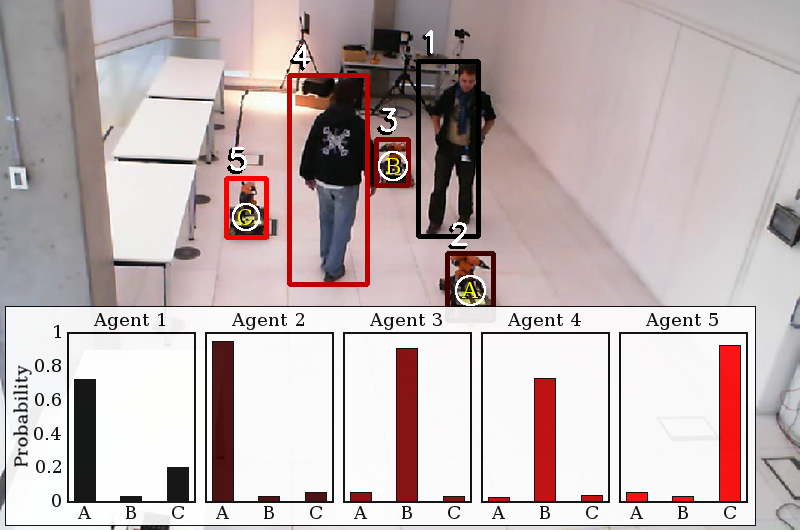
\includegraphics[scale=0.38]{Figures/Motivation.png}
			};
		\end{tikzpicture}
	\end{center}
\end{frame}

\begin{frame}
	\frametitle{Non-Uniform Recursive Grid Representation}
	
	\vspace{0.05cm}
	
	\begin{center}
		\begin{tikzpicture}
			\node at (0,0) [draw=black,ultra thick,inner sep=0pt]
			{
				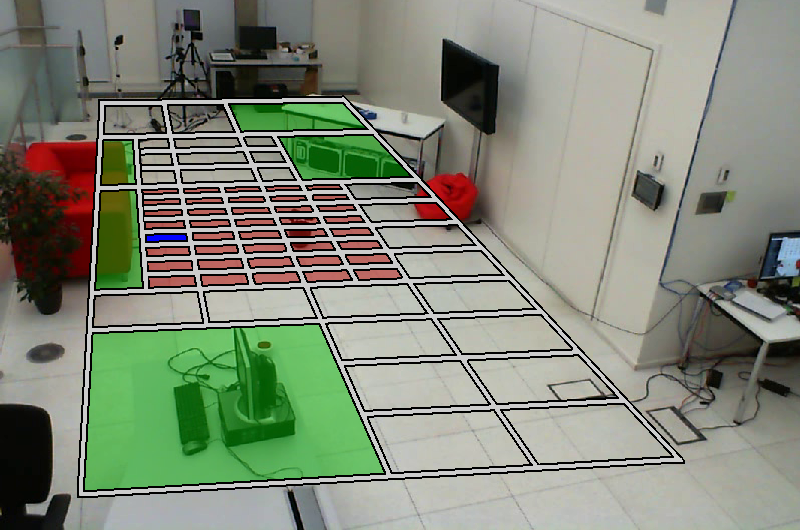
\includegraphics[scale=0.48]{Figures/RecursiveNonUniformGrids.png}
			};
		\end{tikzpicture}
	\end{center}
\end{frame}

\begin{frame}
	\frametitle{Inverse Reinforcement Learning Model}
	
	\vspace{0.05cm}
	
	\begin{center}
		\begin{tikzpicture}
			\node at (0,0) [draw=white,ultra thick,inner sep=0pt]
			{
				\includegraphics[scale=0.275]{Figures/IRL-Model.png}
			};
		\end{tikzpicture}
	\end{center}
\end{frame}
